\documentclass{article}

\usepackage[T1]{fontenc}
\usepackage{graphicx}
\usepackage[a4paper, margin=2cm]{geometry}
\usepackage{lastpage}
\usepackage{fancyhdr}
\usepackage{datetime}
\usepackage{glossaries}

\makeglossaries

\newglossaryentry{gmp}
{
  name=GMP,
  description={Good manufacturing practice, created by the EU and Danish medicines agency.}
}

\newglossaryentry{fdg}{name={FDG},description={[$^{18}$F]Fluorodeoxyglucose, a common radioactive tracer used for PET images}}

\graphicspath{{./figures/}}

\fancyhf{}
\fancyfoot[L]{\today}
\fancyfoot[R]{Page \thepage \, of \pageref{LastPage}}
\pagestyle{fancy}

\author{Christoffer Vilstrup Jensen}
\title{Technical documentation}
\begin{document}


\begin{titlepage}
  \begin{minipage}{0.48\linewidth}
    
\includegraphics[width=0.6\linewidth]{logo.png}
  \end{minipage}
  \begin{minipage}{0.48\linewidth}
    \raggedleft
      
\includegraphics[width=0.6\linewidth]{petlogo_small.png}
  \end{minipage}
  \vspace{1cm}
  \begin{center}
    \Huge Technical documentation and risk assessment for Tracershop \\
    \vspace{1cm}
    \Large Christoffer Vilstrup Jensen\\
  \end{center}
\end{titlepage}

\section*{Resume}
This document describes the current Tracershop ecosystem,
a bookkeeping system for the production of radioactive tracers for clinical procedures produced at Rigshospitalet.
As the system was designed in 2004, the field of Computer Science have moved quite far, this document presents a replacement system with the aims
to improve the user experience, functionality, and improve IT-security.
This document describes a new web interface and makes a risk assessment of the current and the new system.

\section*{Tracershop - Current system}
The original Tracershop was originally produced in 2004. Various people have contributed to the ecosystem over the years,
however active development the system stopped around 2012.
The main functionality of Tracershop is fulfilling the documentations requirements specified by \gls{gmp} in Rigshospitalets production of radioactive Tracers.
Rigshospitalet delivers to many hospitals and scientific institutions,
so it should be considered a important piece of software.\\
The list of customer is not limited to users on the regions intranet, therefore the service needs to be accessible from the internet.\\
The system based around a MySQL 5.1 database running on a openSUSE 11.2 distribution.
The user interface is a  Zope 2-2.13 web interface allowing the users interface with the main database.
There's a dispenser of the tracer, that ensures the dispensed amount tracer and the digital amount of tracer is the same.
The dispenser writes to it own database, which does not support multiple concurrent connections.
A Tracershop component retrieves the data of the dispensed vial by opening the database as a file, seeks to an offset just before the new line was added and
adds an entry in the database. The author of this script no longer works at Rigshospitalet. This solution is highly fragile, as an update to the database would
render the script inoperable as the byte offset would no longer be correct.
In such a case the script would read garbage would not be able to construct a valid entry and thus would mostly likely fail.
At which point the production would have to manually write the data into Tracershops database, which introduces another human error.\\
Due to the nature of the dispenser, a less fragile solution is impossible, it's therefore recommended to replace the dispenser, with one fulfils the requirements of either:
\begin{itemize}
  \item Writes dispensed tracer data to a database that allows multiple connections.
  \item Writes dispensed tracer data to a file.
\end{itemize}
Tracershop software components reached end of life, and as such continued usage is not advised. Tracershop was build with correctness in mind,
however that's no longer sufficient for a good IT product. Sadly IT-criminality is on the rise, as such it necessary to bad actors, even in a low risk system,
such as tracershop.\\
Currently it's the The Department of clinical physiology nuclear medicine which hosts the server.

An overview of the system can be seen in figure \ref{fig:oldsys}.
\begin{figure}[ht]
  \begin{center}
    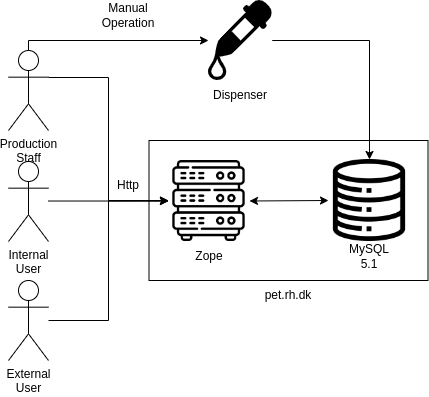
\includegraphics[width=0.6\linewidth]{OldSetup.png}
    \caption{Tracershop system overview}
    \label{fig:oldsys}
  \end{center}
\end{figure}

\subsection*{Abstractions}
Tracershop have two different types of orders. Activity based orders and Injection based orders.
An "Activity Order" is defined as an order, where the user orders an amount of MBq radioactive tracer at a predetermined time slot known as a "deliver time".
Hence it's the user responsibility to account for radioactive decay and order a sufficient amount tracer.
While an injection order consists of a number of injections, and it's Tracershops responsibility to account for any decay between production time and injection time.
Users er limited per user basis which injection tracers they can order.

\subsection*{Requirements}

\begin{itemize}
  \item A user can order radioactive tracer from the internet while not connected to the Capital Region intranet.
  A user can be limited in their selection of tracers and limited time window where such tracers are available for ordering.
  \item A user can review any order they have made, and view batch number of tracer that they have ordered. They cannot view or alter order, which doesn't belong to them.
  \item It's possible to track, which staff member produced which order. A released order must have a valid batch number.
  \item Non authenticated users cannot alter or view information in tracershop.
\end{itemize}

\subsection*{Database layout}
The Tables in the Tracershop main database, note the tables casing does not conform to the snake casing that standard for SQL databases:
\begin{enumerate}
  \item Log - Likely Zope related. No longer in use as the last entry was in 2010-03-18.
  \item MiscData - Likely Zope related. Likely a temporary value container.
  \item Roles - Zope related, defines different user roles in the Tracershop program.
  \item Sessions - Likely Zope related, defines active user sessions.
  \item Tokens - Likely Zope related, Likely defines the length of active sessions.
  \item TracerCustomer - Defines which user have access to order which injection Tracer.
  \item Tracers - Catalog of tracer available in tracershop.
  \item UserRoles - Relates user to a Role from the Role table.The way a web server 
  \item productions - Production of tracers.
  \item storage - Old mails, assumed not in use.
  \item t\_orders - List of injection orders.
\end{enumerate}
The database are not utilizing the foreign key restriction, meaning that the relations are ensured at application level and not the database level.
It's recommend to utilize the these functionality to ensure that the database stays in a valid state.
For instance if a tracer entry is dropped or updated, it may not be possible to determine the tracer of any historic order, that might have used this tracer.\\
Despite Activity orders having a tracer field, this is ignored by the web interface and assumed to be \Gls{fdg}.

\section*{New System}
Tracershop is a system of individual components, so a simple switch of system is not advised, as any of new components would likely contain early adopter errors.
While these errors likely are easy to resolve, they would still take the system down, which is unacceptable.
The best plan of action would be replace each individual component,
and if possible have old component running as a backup in the event that a new component has an error.\\
The largest and easiest to replace component is the web interface, as it can connect to the MySQL database and updates done by the new and old system can co-exists,
as long as the old and the new system follows the same assumptions.\\
Once the basic functionality of a new component is fulfilled and the robustness of the system have been verified. The old system can be retried and
any assumptions held by the old system can be dropped.

\clearpage

\printglossaries
\end{document}